\begin{frame}[allowframebreaks]{Zeit- und Frequenzdomäne}
    \begin{itemize}
        \item{Zeitdomäne}: Horizontale -> diskrete Zeitindizes; Vertikale -> Amplitude
        \item{Frequenzdomäne}: Horizontale -> Frequenz in \textit{Hz}; Vertikale -> Magnitude
        \begin{figure}[H]
            \centering
            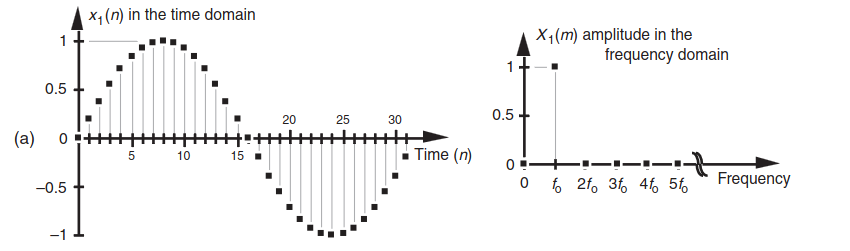
\includegraphics[width=0.6\textwidth]{Graphics/Lyons_time_freq_domain.png.png}
            \caption{
                Gegenüberstellung: Zeit-/Frequenzdomäne einer Sinuswelle
                \citeauthor{lyons2011}, \citeyear{lyons2011}\footcite[Kap. 2]{lyons2011}
            }
        \end{figure}
        \item Umwandlung eines Signals in Zeitdomäne in Frequenzdomäne mithilfe der \textit{Fourier Transformation}:
        \begin{equation}
            X[m] = \sum_{n = 0}^{N - 1}x[n] \cdot e^{\frac{-i2\pi \cdot nm}{N}}
        \end{equation}
    \end{itemize}
\end{frame}